\documentclass[11pt]{article}
\usepackage[spanish]{babel}
\usepackage[utf8]{inputenc}
\usepackage{listings}
\usepackage{graphicx}
\graphicspath{{../Imagenes/}}

\usepackage[paper=portrait, pagesize]{typearea}
\usepackage{titlepic}

%%% Tablas
\usepackage{tabularx}
\usepackage{float}
\usepackage{adjustbox}
\usepackage{booktabs}
\usepackage{multirow}
\renewcommand{\arraystretch}{1.7}

\begin{document}

\begin{titlepage}
\centering
\vspace{4.5cm}
{\scshape\LARGE Descripción inicial del sistema. Modelado de usuarios y escenarios \par}
\vspace{1.5cm}


\includegraphics[width=16cm] {Logo}

\vspace{3cm}
{\scshape\large \par}
\vspace{1cm}

{Miguel Albertí Pons\\
Sofía Almeida Bruno\\
Pedro Manuel Flores Crespo\\
María Victoria Granados Pozo\\
Lidia Martín Chica
\par}

\end{titlepage}


\newpage

\section{Personajes}
%%TABLA JAVI
\begin{table}[H]
  \centering
  \begin{tabular}{p{0.2\linewidth}|p{0.3\linewidth}p{0.475\linewidth}}
    \toprule
    \textbf{Nombre} & Javier Martín Parra &\multirow{4}{*}{\begin{minipage}{1.\textwidth}
\includegraphics[width=0.2\textwidth, height=30mm]{Javier}\end{minipage}}\\
    \textbf{Edad} & 23 & \\
    \textbf{Sexo} & Hombre & \\
    \textbf{Educación} & Graduado en Historia & \\
    \bottomrule
  \end{tabular}

  \begin{tabular}{l}
    \textbf{Contexto de uso} 
  \end{tabular}
  
  \begin{tabular}{p{0.2\linewidth}|p{0.8\linewidth}}
    \toprule
    \textbf{Cuándo} & El domingo, ya que es su día libre en la preparación de las oposiciones\\
    \textbf{Dónde}  & En su casa\\
    \textbf{Tipo de ordenador} & En este caso, utiliza su dispositivo móvil\\
    \bottomrule
  \end{tabular}

  \begin{tabular}{l}
    \textbf{Misión} 
  \end{tabular}
  
  \begin{tabular}{p{0.2\linewidth}|p{0.8\linewidth}}
    \toprule
    \textbf{Objetivo} & Organizar un viaje a Turquía\\
    \textbf{Expectativas}  & Espera aprovechar las experiencias de otros usuarios para que su viaje sea inolvidable \\
    \bottomrule
  \end{tabular}

  \begin{tabular}{l}
    \textbf{Motivación} 
  \end{tabular}

  \begin{tabular}{p{0.2\linewidth}|p{0.8\linewidth}}
    \toprule
    \textbf{Urgencia} & Como quiere realizar el viaje cuando termine las oposiciones, no tiene mucha prisa\\
    \textbf{Deseo}  & Le gustaría hacer este viaje para aprender más sobre el imperio bizantino \\
    \bottomrule
  \end{tabular}

  \begin{tabular}{p{1.028\linewidth}}
    \textbf{Actitud hacia la tecnología}\\
    \midrule
    Ha nacido en la época digital y utiliza con total confianza todo tipo de dispositivos y aplicaciones, tanto nuevas como ya conocidas
  \end{tabular}
\end{table}

\newpage
%%TABLA PEDRO
\begin{table}[H]
  \centering
  \begin{tabular}{p{0.2\linewidth}|p{0.3\linewidth}p{0.475\linewidth}}
    \toprule
    \textbf{Nombre} & Pedro Barranco Sánchez &\multirow{4}{*}{\begin{minipage}{1.\textwidth}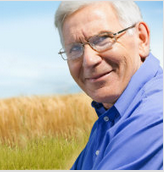
\includegraphics[width=0.2\textwidth, height=30mm]{Pedro}\end{minipage}}\\
    \textbf{Edad} & 73 & \\
    \textbf{Sexo} & Hombre & \\
    \textbf{Educación} & Jubilado & \\
    \bottomrule
  \end{tabular}

  \begin{tabular}{l}
    \textbf{Contexto de uso} 
  \end{tabular}
  
  \begin{tabular}{p{0.2\linewidth}|p{0.8\linewidth}}
    \toprule
    \textbf{Cuándo} & Casi todos los días después de comer\\
    \textbf{Dónde}  & En su casa\\
    \textbf{Tipo de ordenador} & Usa una tablet\\
    \bottomrule
  \end{tabular}

  \begin{tabular}{l}
    \textbf{Misión} 
  \end{tabular}
  
  \begin{tabular}{p{0.2\linewidth}|p{0.8\linewidth}}
    \toprule
    \textbf{Objetivo} & Buscar un regalo para su mujer por el aniversario\\
    \textbf{Expectativas}  & Encontrar un evento cultural en su ciudad, y que llegue el transporte público \\
    \bottomrule
  \end{tabular}

  \begin{tabular}{l}
    \textbf{Motivación} 
  \end{tabular}

  \begin{tabular}{p{0.2\linewidth}|p{0.8\linewidth}}
    \toprule
    \textbf{Urgencia} & No mucha, ya que buscará eventos para todo el mes\\
    \textbf{Deseo}  & Pasar una noche diferente con su mujer \\
    \bottomrule
  \end{tabular}

  \begin{tabular}{p{1.028\linewidth}}
    \textbf{Actitud hacia la tecnología}\\
    \midrule
    No entiende la tablet muy bien, y por eso se pone nervioso cuando no sabe hacer algo
  \end{tabular}
\end{table}


\begin{table}[H]
  \centering
  \begin{tabular}{p{0.2\linewidth}|p{0.3\linewidth}p{0.475\linewidth}}
    \toprule
    \textbf{Nombre} & Ana García Barranco &\multirow{4}{*}{\begin{minipage}{1.\textwidth}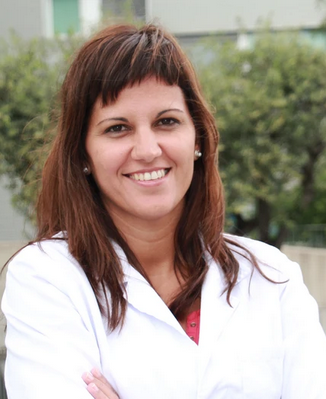
\includegraphics[width=0.2\textwidth, height=30mm]{Ana}\end{minipage}}\\
    \textbf{Edad} & 38 & \\
    \textbf{Sexo} & Mujer & \\
    \textbf{Educación} & Cirujana & \\
    \bottomrule
  \end{tabular}

  \begin{tabular}{l}
    \textbf{Contexto de uso} 
  \end{tabular}
  
  \begin{tabular}{p{0.2\linewidth}|p{0.8\linewidth}}
    \toprule
    \textbf{Cuándo} & En viernes en la guardia del hospital\\
    \textbf{Dónde}  & En el hospital\\
    \textbf{Tipo de ordenador} & Movil personal\\
    \bottomrule
  \end{tabular}

  \begin{tabular}{l}
    \textbf{Misión} 
  \end{tabular}
  
  \begin{tabular}{p{0.2\linewidth}|p{0.8\linewidth}}
    \toprule
    \textbf{Objetivo} & Organizar una actividad familiar para el domingo\\
    \textbf{Expectativas}  & La actividad se realice cerca de su pueblo, y que no tenga un coste elevado \\
    \bottomrule
  \end{tabular}

  \begin{tabular}{l}
    \textbf{Motivación} 
  \end{tabular}

  \begin{tabular}{p{0.2\linewidth}|p{0.8\linewidth}}
    \toprule
    \textbf{Urgencia} & Máxima, porque quiere realizar la actividad este fin de semana.\\
    \textbf{Deseo}  & Disfrutar de un bonito día en familia, y que no le dedique mucho tiempo a encontrar la actividad.\\
    \bottomrule
  \end{tabular}

  \begin{tabular}{p{1.028\linewidth}}
    \textbf{Actitud hacia la tecnología}\\
    \midrule
    Tiene manejo de las tecnologías, pero aún así es precavida.  
  \end{tabular}
\end{table}

%%HAY QUE HACER LAS TABLAS
\newpage
\section{Escenarios}
ESCENARIO 1
Ana quiere realizar una actividad el domingo cerca de su pueblo natal. El viernes al entrar en el trabajo se ha puesto con la aplicación MakeATravel para buscar una plan que cumpla con sus exigencias.
Necesita una actividad adaptada para niños, donde pueda llevar a su hija pequeña, y pasar un gran día en familia.
Gracias a los filtros de la aplicación, puede ver las distintas excursiones que estarán disponibles para ese día, además de información como hora de inicio, precio y la ruta para llegar, podrá ver las opiniones de otros usuarios que ya hayan estado. Factor que hará que, finalmente, elija una excursión por Sierra Nevada.

ESCENARIO 2
Ana llega a su casa el domingo por la noche tras finalizar la excursión y accede en la aplicación para dar una valoración. one una queja sobre la información que se aporta en la actividad, ya que indicaba que la excursión duraría dos horas y han sido tres horas. Además no era apta para su hija ya que era una ruta muy peligrosa para niños.

ESCENARIO 3
Pedro está buscando un regalo de aniversario para su mujer. Después de comer coge la tablet y accede a MakeATravel para buscar algún evento cultural, como por ejemplo un teatro o una opera, que haya en su ciudad. Tras varios días de busqueda encuentra una obra teatral que se realizará a finales de mes. Accede a la información para ver la pagina oficial de la compañia y poder comprar las entradas.

\end{document}
